\documentclass{article}
\usepackage{mathrsfs}
\usepackage{amsmath}
\usepackage{amsthm}
\usepackage{amssymb}
\usepackage{graphicx}
\usepackage{color}
\usepackage{multirow}
\DeclareMathOperator*{\argmax}{argmax}
%\include{macros}
%\usepackage{floatflt}
%\usepackage{graphics}
%\usepackage{epsfig}


\theoremstyle{definition}
\newtheorem{theorem}{Theorem}[section]
\newtheorem{lemma}[theorem]{Lemma}
\newtheorem{proposition}[theorem]{Proposition}
\newtheorem{corollary}[theorem]{Corollary}

\theoremstyle{definition}
\newtheorem*{defition}{Definition}
\newtheorem*{example}{Example}

\theoremstyle{remark}
\newtheorem*{remark}{Remark}
\newtheorem*{note}{Note}
\newtheorem*{exercise}{Exercise}

\setlength{\oddsidemargin}{-0.25 in}
\setlength{\evensidemargin}{-0.25 in} \setlength{\topmargin}{-0.25
in} \setlength{\textwidth}{7 in} \setlength{\textheight}{8.5 in}
\setlength{\headsep}{0.25 in} \setlength{\parindent}{0 in}
\setlength{\parskip}{0.1 in}

\newcommand{\homework}[4]{
\pagestyle{myheadings} \thispagestyle{plain}
\newpage
\setcounter{page}{1} \setcounter{section}{#4} \noindent
\begin{center}
\framebox{ \vbox{\vspace{2mm} \hbox to 6.28in { {\bf
THU-70250043,~Pattern~Recognition~(Spring 2016) \hfill Homework: 3} }
\vspace{6mm} \hbox to 6.28in { {\Large \hfill #1 \hfill} }
\vspace{6mm} \hbox to 6.28in { {\it Lecturer: #2 \hfill} }
\vspace{2mm} \hbox to 6.28in { {\it Student: #3 \hfill} }
\vspace{2mm} } }
\end{center}
\markboth{#1}{#1} \vspace*{4mm} }


\begin{document}

\homework{Gaussian Mixture Model and Expectation Maximization Algorithm}{Changshui Zhang
\hspace{5mm} {\tt zcs@mail.tsinghua.edu.cn}}{Qingfu Wen \hspace{5mm} {\tt
wqf15@mails.tsinghua.edu.cn } }{8}

%%%%%%%%%%%%%%%%%%%%%%%%%%%%%%%%%%%%%%%%%%%%%%%%%%%%%%%%%%%%%%%%%%%%
% Section 2.  Problem
%%%%%%%%%%%%%%%%%%%%%%%%%%%%%%%%%%%%%%%%%%%%%%%%%%%%%%%%%%%%%%%%%%%%
\section*{EM and Gradient Descent}
In this problem you will investigate connections between the EM algorithm and gradient descent. Consider a GMM where
$\Sigma_k=\sigma_k^2I$, i.e., the covariances are spherical but of different spread. Moreover, suppose the mixture weight
$\pi_k$ is known. The log likelihood then is
\[
l\left(\{\mu_k,\sigma_k^2\}_{k=1}^K\right) = \sum_{i=1}^n\log\left(\sum_{k=1}^K\pi_k~N(x_i|\mu_k,\sigma_k^2I)\right).
\]
A maximization algorithm based on gradient descent is as follows:
\begin{itemize}
  \item Initialize $\mu_k$ and $\sigma_k^2$, $k \in \{1,\cdots ,K\}$. Set the iteration counter t=1.
  \item Repeat the following until convergence:
  \begin{itemize}
    \item For $k=1,\cdots ,K$,
    \[
    \mu_k^{(t+1)}\leftarrow\mu_k^{(t)}+\eta_k^{(t)}\triangledown_{\mu_k}l\left(\{\mu_k^{(t)},(\sigma_k ^2)^{(t)}\}_{k=1}^K\right)
    \]
    \item For $k=1,\cdots ,K$,
    \[
    (\sigma_k ^2)^{(t+1)} \leftarrow (\sigma_k ^2)^{(t)}+s_k^{(t)}\triangledown_{\sigma_k^2}l\left(\{\mu_k^{(t+1)},(\sigma_k ^2)^{(t)}\}_{k=1}^K\right)
    \]
    \item Increase the iteration counter $t\leftarrow t+1$
  \end{itemize}
\end{itemize}
Show that with properly chosen step size $\eta_k^{(t)}$ and $s_k^{(t)}$, the above gradient descent algorithm is equivalent to the following modified EM algorithm:
\begin{itemize}
  \item Initialize $\mu_k$ and $\sigma_k^2$, $k \in \{1,\cdots ,K\}$. Set the iteration counter t=1.
  \item Repeat the following until convergence:
  \begin{itemize}
    \item E-step:
    \[
    \tilde{z}_{ik}^{(t+0.5)} \leftarrow Prob\left(x_i\in cluster_k | \{(\mu_j^{(t)},(\sigma_j^2)^{(t)})\}_{j=1}^K,x_i\right),
    \]
    \item M-step:
    \[
    \{\mu_k^{(t+1)}\}_{k=1}^K \leftarrow arg\max_{\{\mu_k\}_{k=1}^K} \sum_{i=1}^n\sum_{k=1}^K \tilde{z}_{ik}^{(t+0.5)} \left(\log~N(x_i|\mu_k,(\sigma_k^2)^{(t)}I)+\log\pi_k\right)
    \]
    \item E-step:
    \[
    \tilde{z}_{ik}^{(t+1)} \leftarrow Prob\left(x_i \in cluster_k|\{(\mu_j^{(t+1)},(\sigma_j^2)^{(t)})\}_{j=1}^K,x_i\right),
    \]
    \item M-step:
    \[
    \{(\sigma_k^2)^{(t+1)}\}_{k=1}^K \leftarrow arg \max_{\{\sigma_k\}_{k=1}^K} \sum_{i=1}^n \sum_{k=1}^K \tilde{z}_{ik}^{(t+1)} \left(\log~N(x_i|\mu_k^{(t+1)},\sigma_k^2 I)+\log \pi_k \right)
    \]
    \item Increase the iteration counter $t\leftarrow t+1$
  \end{itemize}
\end{itemize}
The main modification is inserting an extra E-step between the M-step for $\mu_k$'s and the M-step for $\sigma_k^2$'s.

\emph{\textbf{SOLUTION:}}\\
In EM algorithm,
\[
\tilde{z}_{ik} = \frac{\pi_k~N(x_i|\mu_k,\sigma_k^2I)}{\sum_{j=1}^K\pi_k~N(x_i|\mu_j,\sigma_j^2I)}
\]
\begin{equation}\nonumber
\mu_k^{(t+1)} = arg\max_{\{\mu_k\}_{k=1}^K} \sum_{i=1}^n\sum_{k=1}^K \tilde{z}_{ik}^{(t+0.5)} \left(\log~N(x_i|\mu_k,(\sigma_k^2)^{(t)}I)+\log\pi_k\right)
\end{equation}
Set the derivative to be 0
\begin{equation}\nonumber
\frac{\partial\left[ \sum_{i=1}^n\sum_{k=1}^K \tilde{z}_{ik}^{(t+0.5)} \left(\log~N(x_i|\mu_k,(\sigma_k^2)^{(t)}I)+\log\pi_k\right)\right]}{\partial \mu_k} = 0
\end{equation}
Then we can get
\begin{equation}\nonumber
\mu_k^{(t+1)} = \frac{\sum_{i=1}^n \tilde{z}_{ik}^{(t+0.5)}x_i}{\sum_{i=1}^n \tilde{z}_{ik}^{(t+0.5)}}
\end{equation}
Similarly, we can get
\begin{equation}\nonumber
(\delta_k^2)^{(t+1)} = \frac{\sum_{i=1}^n \tilde{z}_{ik}^{(t+1)}(x_i-\mu_k^{(t+1)})^2}{\sum_{i=1}^n \tilde{z}_{ik}^{(t+1)}}
\end{equation}

In gradient descent algorithm, we have
\[
l\left(\{\mu_k,\sigma_k^2\}_{k=1}^K\right) = \sum_{i=1}^n\log\left(\sum_{k=1}^K\pi_k~N(x_i|\mu_k,\sigma_k^2I)\right).
\]
\begin{equation}\nonumber
\begin{aligned}
\triangledown_{\mu_k}l\left(\{\mu_k,\sigma_k^2\}_{k=1}^K\right) &= \sum_{i=1}^n \frac{\pi_k~N(x_i|\mu_k,\sigma_k^2I)}{\sum_{j=1}^K\pi_k~N(x_i|\mu_j,\sigma_j^2I)}\frac{x_i-\mu_k}{\delta_k^2}\\
&= \sum_{i=1}^n  \frac{\tilde{z}_{ik}}{\delta_k^2}(x_i-\mu_k)
\end{aligned}
\end{equation}

\begin{equation}\nonumber
\begin{aligned}
\triangledown_{\delta_k^2}l\left(\{\mu_k,\sigma_k^2\}_{k=1}^K\right)
&= \sum_{i=1}^n \frac{\pi_k~N(x_i|\mu_k,\sigma_k^2I)}{\sum_{j=1}^K\pi_k~N(x_i|\mu_j,\sigma_j^2I)}[\frac{(x_i-\mu_k)^2}{2(\delta_k^2)^2}-\frac{1}{2\delta_k^2}]
\\
&= \sum_{i=1}^n \tilde{z}_{ik}[\frac{(x_i-\mu_k)^2}{2(\delta_k^2)^2}-\frac{1}{2\delta_k^2}]
\end{aligned}
\end{equation}

Set $\eta_k^{(t)}=\frac{(\delta_k^2)^{(t)}}{\sum_{i=1}^n \tilde{z}_{ik}^{(t+0.5)}}$, then
\begin{equation}\nonumber
\begin{aligned}
\mu_k^{(t+1)}&=\mu_k^{(t)}+\eta_k^{(t)}\triangledown_{\mu_k}l\left(\{\mu_k^{(t)},(\sigma_k ^2)^{(t)}\}_{k=1}^K\right)\\
&=\mu_k^{(t)}+\frac{(\delta_k^2)^{(t)}}{\sum_{i=1}^n \tilde{z}_{ik}^{(t+0.5)}} \frac{\sum_{i=1}^n\tilde{z}_{ik}^{(t+0.5)}}{(\delta_k^2)^{(t)}}(x_i-\mu_k)\\
&=\frac{\sum_{i=1}^n \tilde{z}_{ik}^{(t+0.5)}x_i}{\sum_{i=1}^n \tilde{z}_{ik}^{(t+0.5)}}
\end{aligned}
\end{equation}

Set $s_k^{(t)}=\frac{2[(\delta_k^2)^{(t)}]^2}{\sum_{i=1}^n \tilde{z}_{ik}^{(t+1)}}$, then
\begin{equation}\nonumber
\begin{aligned}
(\delta_k^2)^{(t+1)} &= (\sigma_k ^2)^{(t)}+s_k^{(t)}\triangledown_{\sigma_k^2}l\left(\{\mu_k^{(t+1)},(\sigma_k ^2)^{(t)}\}_{k=1}^K\right) \\
&= (\sigma_k ^2)^{(t)}+\frac{2[(\delta_k^2)^{(t)}]^2}{\sum_{i=1}^n \tilde{z}_{ik}^{(t+1)}}\sum_{i=1}^n \tilde{z}_{ik}^{(t+1)}[\frac{(x_i-\mu_k^{(t+1)})^2}{2((\delta_k^2)^{(t)})^2}-\frac{1}{2(\delta_k^2)^{(t)}}]\\
&= \frac{\sum_{i=1}^n \tilde{z}_{ik}^{(t+1)}(x_i-\mu_k^{(t+1)})^2}{\sum_{i=1}^n \tilde{z}_{ik}^{(t+1)}}
\end{aligned}
\end{equation}
\section*{EM for MAP Estimation}
The EM algorithm that we talked about in class was for solving a maximum likelihood estimation problem in which we wished to maximize
\begin{equation}
  \prod_{i = 1}^mp(x^{(i)};\theta) = \prod_{i = 1}^m \sum_{z^{(i)}}p(x^{(i)},z^{(i)};\theta)
\end{equation}
where the $z^{(i)}$'s were latent random variables. Suppose we are working in a Bayesian framework, and wanted to find the MAP estimate of the parameters $\theta$ by maximizing
\begin{equation}
  (\prod_{i = 1}^mp(x^{(i)};\theta))p(\theta) = (\prod_{i = 1}^m \sum_{z^{(i)}}p(x^{(i)},z^{(i)}|\theta))p(\theta)
\end{equation}
Here, $p(\theta)$ is our prior on the parameters. Generalize the EM algorithm to work for MAP
estimation. You may assume that $log\;p(x,z|\theta)$ and $log\;p(\theta)$ are both concave in $\theta$, so
that the M-step is tractable if it requires only maximizing a linear combination of these
quantities. (This roughly corresponds to assuming that MAP estimation is tractable when
$x, z$ is fully observed, just like in the frequentist case where we considered examples in
which maximum likelihood estimation was easy if $x, z$ was fully observed.)

Make sure your M-step is tractable, and also prove that $(\prod_{i = 1}^mp(x^{(i)};\theta))p(\theta)$(viewed as a
function of $\theta$) monotonically increases with each iteration of your algorithm.

\emph{\textbf{SOLUTION:}}\\
\begin{equation}\nonumber
\begin{aligned}
\ln(\prod_{i = 1}^mp(x^{(i)};\theta))p(\theta) &= \ln p(\theta)+ \sum_{i=1}^m\ln p(x^{(i)};\theta)\\
 &= \ln p(\theta)+ \sum_{i=1}^m\ln \sum_{z^{(i)}}p(x^{(i)},z^{(i)}|\theta)\\
 &= \ln p(\theta)+ \sum_{i=1}^m\ln \sum_{z^{(i)}}Q_i(z^{(i)})\frac{p(x^{(i)},z^{(i)}|\theta)}{Q_i(z^{(i)})}\\
 &\geq \ln p(\theta)+ \sum_{i=1}^m\sum_{z^{(i)}}Q_i(z^{(i)})\ln\frac{p(x^{(i)},z^{(i)}|\theta)}{Q_i(z^{(i)})}\\
\end{aligned}
\end{equation}
From above equation, give the E-step:
\[Q_i(z^{(i)})=p(z^{(i)}|x^{(i)};\theta)\]
At the M-step, we need to maximize:
\[\theta = \argmax_{\theta}\left(\ln p(\theta)+ \sum_{i=1}^m\sum_{z^{(i)}}Q_i(z^{(i)})\ln\frac{p(x^{(i)},z^{(i)}|\theta)}{Q_i(z^{(i)})}\right)\]
Now prove $(\prod_{i = 1}^mp(x^{(i)};\theta))p(\theta)$ increases with each iteration. Set
\[L(\theta) = \ln(\prod_{i = 1}^mp(x^{(i)};\theta))p(\theta)\]
$\theta^{(t)},\theta^{(t+1)}$ is the $t, t+1$ iteration result of EM algorithm. At the E-step of the $t$-th iteration,
\[Q_i^{(t)}(z^{(i)})=p(z^{(i)}|x^{(i)};\theta)\]
that means Jensen inequality is tight
\[L(\theta^{(t)})=\sum_{i=1}^m\sum_{z^{(i)}}Q_i^{(t)}(z^{(i)})\ln\frac{p(x^{(i)},z^{(i)}|\theta^{(t)})}{Q_i^{(t)}(z^{(i)})}\]
Then do the M-step, derive $L(\theta)$ and we get $\theta^{(t+1)}$
\begin{equation}\nonumber
\begin{aligned}
L(\theta^{(t+1)})
&\geq \ln p(\theta^{(t+1)})+ \sum_{i=1}^m\sum_{z^{(i)}}Q_i^{(t)}(z^{(i)})\ln\frac{p(x^{(i)},z^{(i)}|\theta^{(t+1)})}{Q_i^{(t)}(z^{(i)})}\\
&\geq\ln p(\theta^{(t)})+ \sum_{i=1}^m\sum_{z^{(i)}}Q_i^{(t)}(z^{(i)})\ln\frac{p(x^{(i)},z^{(i)}|\theta^{(t)})}{Q_i^{(t)}(z^{(i)})}\\
 &= L(\theta^{(t)})
\end{aligned}
\end{equation}
\section*{EM Application}
Consider the following problem. There are $P$ papers submitted to a machine learning
conference. Each of $R$ reviewers reads each paper, and gives it a score indicating how good
he/she thought that paper was. We let $x^{(pr)}$ denote the score that reviewer $r$ gave to paper
$p$. A high score means the reviewer liked the paper, and represents a recommendation from
that reviewer that it be accepted for the conference. A low score means the reviewer did
not like the paper.

We imagine that each paper has some ``intrinsic'' true value that we denote by $\mu_p$, where a
large value means it's a good paper. Each reviewer is trying to estimate, based on reading
the paper, what $\mu_p$ is; the score reported $x^{(pr)}$ is then reviewer $r$'s guess of $\mu_p$.

However, some reviewers are just generally inclined to think all papers are good and tend
to give all papers high scores; other reviewers may be particularly nasty and tend to give
low scores to everything. (Similarly, different reviewers may have different amounts of
variance in the way they review papers, making some reviewers more consistent/reliable
than others.) We let $\nu_r$ denote the ``bias'' of reviewer $r$. A reviewer with bias $\nu_r$ is one
whose scores generally tend to be $\nu_r$ higher than they should be.

All sorts of different random factors influence the reviewing process, and hence we will use
a model that incorporates several sources of noise. Specifically, we assume that reviewers'
scores are generated by a random process given as follows:
\begin{equation}
  \begin{aligned}
  y^{(pr)} &\sim \mathcal{N}(\mu_p, \sigma_p^2) \\
  z^{(pr)} &\sim \mathcal{N}(\nu_r, \tau_r^2) \\
  x^{(pr)} |y^{(pr)}, z^{(pr)} &\sim \mathcal{N}(y^{(pr)} + z^{(pr)}, \sigma^2)
  \end{aligned}
\end{equation}
The variables $y^{(pr)}$ and $z^{(pr)}$ are independent; the variables $(x, y, z)$ for different paper-
reviewer pairs are also jointly independent. Also, we only ever observe the $x^{(pr)}$'s; thus,
the $y^{(pr)}$'s and $z^{(pr)}$'s are all latent random variables.

We would like to estimate the parameters $\mu_p, \sigma_p^2, \nu_r; \tau_r^2$. If we obtain good estimates of
the papers' ``intrinsic'' values $\mu_p$, these can then be used to make acceptance/rejection
decisions for the conference.

We will estimate the parameters by maximizing the marginal likelihood of the data $\{x^{(pr)}; p =
1, \ldots, P, r = 1, \ldots, R\}$. This problem has latent variables $y^{(pr)}$ and $z^{(pr)}$, and the maximum likelihood problem cannot be solved in closed form. So, we will use EM. Your
task is to derive the EM update equations. Your final E and M step updates should
consist only of addition/subtraction/multiplication/division/log/exp/sqrt of scalars; and
addition/subtraction/multiplication/inverse/determinant of matrices. For simplicity, you
need to treat only $\{\mu_p, \sigma_p^2; p = 1, \ldots, P\}$ and $\{\nu_r, \tau_r^2; r = 1, \ldots, R\}$ as parameters. I.e. treat
$\sigma^2$ (the conditional variance of $x^{(pr)}$ given $y^{(pr)}$ and $z^{(pr)}$) as a fixed, known constant.

\begin{itemize}
  \item In this part, we will derive the E-step:
    \begin{itemize}
      \item The joint distribution $p(y^{(pr)}, z^{(pr)}, x^{(pr)})$ has the form of a multivariate Gaussian
density. Find its associated mean vector and covariance matrix in terms of the parameters $\mu_p, \sigma_p^2, \nu_r, \tau_r^2$ and $\sigma^2$.
      \item Derive an expression for $Q_{pr}(y^{(pr)}, z^{(pr)}) = p(y^{(pr)}, z^{(pr)}|x^{(pr)})$ (E-step), using the
rules for conditioning on subsets of jointly Gaussian random variables.
    \end{itemize}
  \item Derive the M-step updates to the parameters $\{\mu_p, \sigma_p^2, \nu_r, \tau_r^2\}$
\end{itemize}
\emph{\textbf{SOLUTION:}}\\

define $\theta$ as all parameters that need to estimate, we get get EM step as follow:\\
\textbf{E-step:} $ Q_{pr}(y^{(pr)},z^{(pr)})= p(y^{(pr)},z^{(pr)}|x^{(pr)};\theta)$\\
\textbf{M-step:} $ \theta= arg\max_{\theta}\sum_{p=1}^{P}\sum_{r=1}^{R}E_{Q_{pr}}\log p(x^{(pr)},y^{(pr)},z^{(pr)};\theta)$
we can compute $p(x^{(pr)},y^{(pr)},z^{(pr)})$:
\[p(x^{(pr)},y^{(pr)},z^{(pr)})=p(y^{(pr)},z^{(pr)})p(x^{(pr)}|y^{(pr)},z^{(pr)})=p(y^{(pr)})p(z^{(pr)})p(x^{(pr)}|y^{(pr)},z^{(pr)})\]
From this, the joint distribution $p(x^{(pr)},y^{(pr)},z^{(pr)}$ is a kind of Gaussian distribution.\\
we can rewrite $x^{(pr)}=y^{(pr)}+z^{(pr)}+\epsilon^{(pr)}$, where $\epsilon^{(pr)}\sim N(0,\sigma^2)$.
\begin{equation}\nonumber
\begin{aligned}
E[x^{(pr)}]&=E[y^{(pr)}+z^{(pr)}+\epsilon^{(pr)}]\\
&=E[y^{(pr)}]+E[z^{(pr)}]+E[\epsilon^{(pr)}]\\
&=\mu_p+\nu_r+0\\
&=\mu_p+\nu_r
\end{aligned}
\end{equation}
\begin{equation}\nonumber
\begin{aligned}
Var[x^{(pr)}]&=Var[y^{(pr)}+z^{(pr)}+\epsilon^{(pr)}]\\
&=Var[y^{(pr)}]+Var[z^{(pr)}]+Var[\epsilon^{(pr)}]\\
&=\sigma_p^2+\tau_r^2+\sigma^2
\end{aligned}
\end{equation}
\begin{equation}\nonumber
\begin{aligned}
Cov[x^{(pr)},y^{(pr)}]&=Cov[y^{(pr)},x^{(pr)}]\\
&=Cov[y^{(pr)}+z^{(pr)}+\epsilon^{(pr)},y^{(pr)}]\\
&=Cov[y^{(pr)},y^{(pr)}]+Cov[z^{(pr)},y^{(pr)}]+Cov[\epsilon^{(pr)},y^{(pr)}]\\
&=\sigma_p^2
\end{aligned}
\end{equation}
\begin{equation}\nonumber
\begin{aligned}
Cov[x^{(pr)},z^{(pr)}]&=Cov[z^{(pr)},x^{(pr)}]\\
&=Cov[y^{(pr)}+z^{(pr)}+\epsilon^{(pr)},z^{(pr)}]\\
&=Cov[y^{(pr)},z^{(pr)}]+Cov[z^{(pr)},z^{(pr)}]+Cov[\epsilon^{(pr)},z^{(pr)}]\\
&=\tau_r^2
\end{aligned}
\end{equation}
Thus,$p(y^{(pr)}, z^{(pr)}, x^{(pr)})\sim N(\begin{bmatrix}\mu_p\\\nu_r\\\mu_p+\nu_r\end{bmatrix},\begin{bmatrix}\sigma_p^2&0&\sigma_p^2\\
0&\tau_r^2&\tau_r^2\\ \sigma_p^2&\tau_r^2&\sigma_p^2+\tau_r^2+\sigma^2\end{bmatrix})$\\
\\
\\
\textbf{E-step:}\\
\[Q_{pr}(y^{(pr)}, z^{(pr)}) = p(y^{(pr)}, z^{(pr)}|x^{(pr)})=N(\begin{bmatrix}\mu_{pr,Y}\\\mu_{pr,Z}\end{bmatrix},\begin{bmatrix}\sum_{pr,YY}&\sum_{pr,YZ}\\
\sum_{pr,ZY}&\sum_{pr,ZZ}\end{bmatrix})\]

\begin{equation}
\begin{bmatrix}\mu_{pr,Y}\\\mu_{pr,Z}\end{bmatrix} = \begin{bmatrix}\mu_p+\frac{\sigma_p^2}{\sigma_p^2+\tau_r^2+\sigma^2}(x^{(pr)}-\mu_p-\tau_r)\\
\tau_r+\frac{\tau_r^2}{\sigma_p^2+\tau_r^2+\sigma^2}(x^{(pr)}-\mu_p-\tau_r)\end{bmatrix}
\end{equation}

\begin{equation}
\begin{bmatrix}\sum_{pr,YY}&\sum_{pr,YZ}\\
\sum_{pr,ZY}&\sum_{pr,ZZ}\end{bmatrix} = \frac{1}{\sigma_p^2+\tau_r^2+\sigma^2} \begin{bmatrix}\mu_p^2(\sigma^2+\tau_r^2)&-\mu_p^2\tau_r^2\\
- \mu_p^2\tau_r^2&\tau_r^2(\sigma^2+\mu_p^2)\end{bmatrix}
\end{equation}

\textbf{M-step:}\\
\begin{equation}\nonumber
\begin{aligned}
\theta &= arg\max_{\theta}\sum_{p=1}^{P}\sum_{r=1}^{R}E_{Q_{pr}}\log p(x^{(pr)},y^{(pr)},z^{(pr)};\theta)\\
&=arg\max_{\theta}\sum_{p=1}^{P}\sum_{r=1}^{R}E_{Q_{pr}}\log
\left[
\frac{1}{\sqrt{2\pi}\sigma}e^{-\frac{(x^{(pr)}-y^{(pr)}-z^{(pr)})^2}{2\sigma^2}}
\frac{1}{\sqrt{2\pi}\sigma_p}e^{-\frac{(y^{(pr)}-\mu_p)^2}{2\sigma_p^2}}
\frac{1}{\sqrt{2\pi}\tau_r}e^{-\frac{(z^{(pr)}-\nu_r)^2}{2\tau_r^2}}\right]\\
&=arg\max_{\theta}\sum_{p=1}^{P}\sum_{r=1}^{R}E_{Q_{pr}}
\left[
\log\frac{1}{\sigma_p\tau_r}-\frac{1}{2\sigma_p^2}((y^{(pr)})^2-2y^{(pr)}\mu_p+\mu_p^2)
-\frac{1}{2\tau_r^2}((z^{(pr)})^2-2z^{(pr)}\nu_r+\nu_r^2)
\right]\\
&=arg\max_{\theta}\sum_{p=1}^{P}\sum_{r=1}^{R}
\left[
\log\frac{1}{\sigma_p\tau_r}-\frac{1}{2\sigma_p^2}(E_Q[(y^{(pr)})^2]-2E_Q[y^{(pr)}]\mu_p+\mu_p^2)
-\frac{1}{2\tau_r^2}(E_Q[(z^{(pr)})^2]-2E_Q[z^{(pr)}]\nu_r+\nu_r^2)
\right]
\end{aligned}
\end{equation}
\[-\frac{1}{2\sigma_p^2}\sum_{r=1}^{R}(2\mu_p-2E_Q[y^{(pr)}])=0 \Rightarrow \mu_p=\frac{1}{R}\sum_{r=1}^{R}E_Q[y^{(pr)}]\]
\[-\frac{1}{2\tau_r^2}\sum_{p=1}^{P}(2\nu_r-2E_Q[z^{(pr)}])=0 \Rightarrow \nu_r=\frac{1}{P}\sum_{p=1}^{P}E_Q[z^{(pr)}]\]
\[\sigma_p=\frac{1}{R}\sum_{r=1}^{R}(E_Q[(y^{(pr)})^2]-2E_Q[y^{(pr)}]\mu_p+\mu_p^2)\]
\[\tau_r^2=\frac{1}{P}\sum_{p=1}^{P}(E_Q[(z^{(pr)})^2]-2E_Q[z^{(pr)}]\nu_r+\nu_r^2)]\]
\section*{Programming 1}
\begin{table}
\centering
\begin{tabular}{|c|c|c|c|c|c|c|c|}
\hline
\multirow{2}{*}{Points} & \multicolumn{3}{|c|}{$\omega_1$} & \multicolumn{3}{|c|}{$\omega_2$} \\
\cline{2-7}
& $x_1$ & $x_2$ & $x_3$ & $x_1$ & $x_2$ & $x_3$ \\
\hline
1 & 0.42 & -0.087 & 0.58 & -0.4 & 0.58 & 0.089\\
\hline
2 & -0.2 & -3.3 & -3.4 & -0.31 & 0.27 & -0.04\\
\hline
3 & 1.3 & -0.32 & 1.7 & 0.38 & 0.055 & -0.035\\
\hline
4 & 0.39 & 0.71 & 0.23 & -0.15 & 0.53 & 0.011\\
\hline
5 & -1.6 & -5.3 & -0.15 & -0.35 & 0.47 & 0.034\\
\hline
6 & -0.029 & 0.89 & -4.7 & 0.17 & 0.69 & 0.1\\
\hline
7 & -0.23 & 1.9 & 2.2 & -0.011 & 0.55 & -0.18\\
\hline
8 & 0.27 & -0.3 & -0.87 & -0.27 & 0.61 & 0.12\\
\hline
9 & -1.9 & 0.76 & -2.1 & -0.065 & 0.49 & 0.0012\\
\hline
10 & 0.87 & -1.0 & -2.6 & -0.12 & 0.054 & -0.063\\
\hline

\end{tabular}
\caption{Data for Programming 1}
\end{table}

Suppose we know that the ten data points in category $\omega_1$ in the table above come
from a three-dimensional Gaussian. Suppose, however, that we do not have access to
the $x_3$ components for the even-numbered data points.
\begin{itemize}
  \item Write an EM program to estimate the mean and covariance of the distribution.
Start your estimate with $\mu_0 = 0$ and $\Sigma_0 = I$, the three-dimensional identity
matrix.
  \item Compare your final estimate with that for the case when there is no missing data
\end{itemize}
\emph{\textbf{SOLUTION:}}
\begin{table}[!htp]
\centering
\begin{tabular}{|c|c|c|}
\hline
   & mean & cov \\
\hline
EM &$[-0.0709 -0.6047 ~~0.3940]$& $\begin{bmatrix} 0.9062   &  0.5678  &  0.6741\\
    0.5678  &   4.2007   &   0.3181\\
    0.6741  &     0.3181   &   4.3197\end{bmatrix}$\\
\hline
real &$[-0.0709 -0.6047 -0.9110]$& $\begin{bmatrix}0.9062   &  0.5678   &  0.3941\\
    0.5678 &    4.2007  &   0.7337\\
    0.3941  &   0.7337  &   4.5419\end{bmatrix}$\\
\hline
\end{tabular}
\end{table}

Suppose we know that the ten data points in category $\omega_2$ in the table above
come from a three-dimensional uniform distribution $p(x|\omega_2) \sim U(x_l, x_u)$. Suppose,
however, that we do not have access to the $x_3$ components for the even-numbered
data points.

\begin{itemize}
  \item Write an EM program to estimate the six scalars comprising $x_l$ and $x_u$ of the distribution.
Start your estimate with $x_l = (-2, -2, -2)^t$ and $x_u = (+2, +2, +2)^t$.
  \item Compare your final estimate with that for the case when there is no missing data.
\end{itemize}

\section*{Programming 2}
Consider the case that the hidden variable $y \in \{1, ..., m\}$ is discrete while the visible variable $x \in R^d$
is continuous. In other words, we consider mixture models of the form
\begin{equation}
  p(x) = \sum_{j = 1}^m p(x|y = j)p(y=j)
\end{equation}
We assume throughout that $x$ is conditionally Gaussian in the sense that $x \sim \mathcal{N}(\mu_j
, \Sigma_j)$ when $y = j$.

We have provided you with the EM code for mixture of Gaussians (with visualization).
The command to run is.

$[\text{param},\text{history},\text{ll}] = \text{em}\_\text{mix}(\text{data,m,eps})$;

where the input points are given as rows of \textbf{data}, \textbf{m} is the number of components in the
estimated mixture, and \textbf{eps} determines the stopping criteria of EM: the algorithm stops
when the relative change in log-likelihood falls below eps. In the output, \textbf{param} is a cell
array with m elements. Each element is a structure with the following fields:

mean - the resulting mean of the Gaussian component,

cov - the resulting covariance matrix of the component,

p - the resulting estimate of the mixing parameter.

The value of param is updated after every iteration of EM; the output argument history
contains copies of these subsequent values of param and allows to analyze our experiments.
Finally, ll is the vector where the t-th element is the value of the log-likelihood of the data
after t iterations (i.e. the last element is the final log-likelihood of the fitted mixture of
Gaussians).

To overcome any numerical problems the code involves (slight) regularization. Specifically,
the M-step of the EM algorithm solves a regularized weighted log-likelihood problem, where
the prior distribution over the mixing proportions is a Dirichlet and the prior over each
covariance matrix is a Wishart. The equivalent sample size is set to one. The returned log-likelihood
values include the regularization penalties (log-priors). See the code for details
if you wish to change any of these settings.

\begin{itemize}
  \item Run the EM algorithm based on data2 provided by hw5em2.mat with m =
2, 3, 4, 5 components. Select the appropriate model (number of components) and give reasons for your choice. Note that you may have to rerun the algorithm a few times
(and select the model with the highest log-likelihood) for each choice of m as EM can
sometimes get stuck in a local minimum. Is the model selection result sensible based
on what you would expect visually? Why or why not?
  \item Modify the M-step of the EM code so that the covariance matrices of
the Gaussian components are constrained to be equal. Give detailed derivation. Rerun the code and then select a appropriate model. Would we select a different number of components in this case?
%Rerun the model selection
%problem using BIC as the selection criterion. Would we select a different number of
%components in this case?

Notes: for the above two questions you are encouraged to google ``BIC'' to help you with the model selection process. Of course other criteria are welcomed as long as you give convincing reasons.
\end{itemize}
\emph{\textbf{SOLUTION:}}
\begin{itemize}
\item
\begin{table}[!htp]
\centering
\begin{tabular}{|c|c|}
\hline
 m & BIC \\
\hline
2 & 8653.9 \\
\hline
3 & 8498.5 \\
\hline
4 & 8343.6 \\
\hline
5 & 8391.9 \\
\hline
\end{tabular}
\end{table}

$BIC = -2*log-likehood + (m*d+m*\frac{d(d+1)}{2}+m)*\ln n$, from the above table, we can see that when $m=4$, we have lowest BIC. Thus, 4 components is the best choice.
\begin{figure}[!htbp]
  \centering
  % Requires \usepackage{graphicx}
  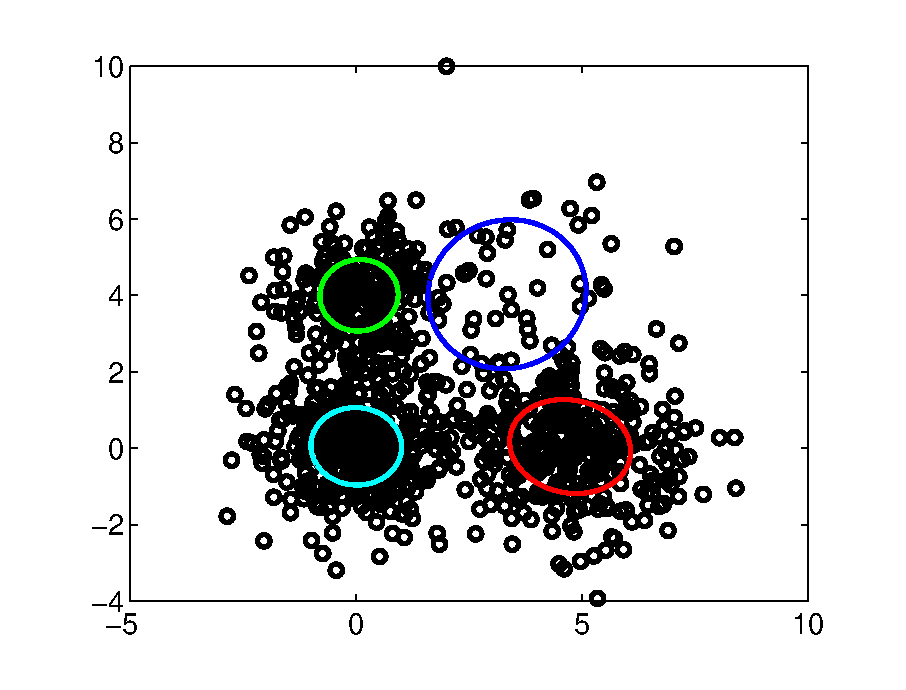
\includegraphics[width=3.5in]{1.eps}\\
\end{figure}

\item

With the covariance matrices of the Gaussian components constrained to be equal, we can calculate the covariance matrix
\[
\Sigma^{(k+1)}=\frac{1}{n}\sum_{i=1}^n\sum_{j=1}^m p(j|i)(x_i-\mu_j^{(k+1)})(x_i-\mu_j^{(k+1)})'\]
$BIC = -2*log-likehood + (m*d+\frac{d(d+1)}{2}+m)*\ln n$.\\
\begin{table}[!htp]
\centering
\begin{tabular}{|c|c|}
\hline
 m & BIC \\
\hline
2 & 8583.6 \\
\hline
3 & 8428.2 \\
\hline
4 & 8458.5 \\
\hline
5 & 8494.4 \\
\hline
\end{tabular}
\end{table}
From the above table, we can see that when $m=3$, we have lowest BIC. Thus, 3 components is the best choice.
\begin{figure}[!htbp]
  \centering
  % Requires \usepackage{graphicx}
  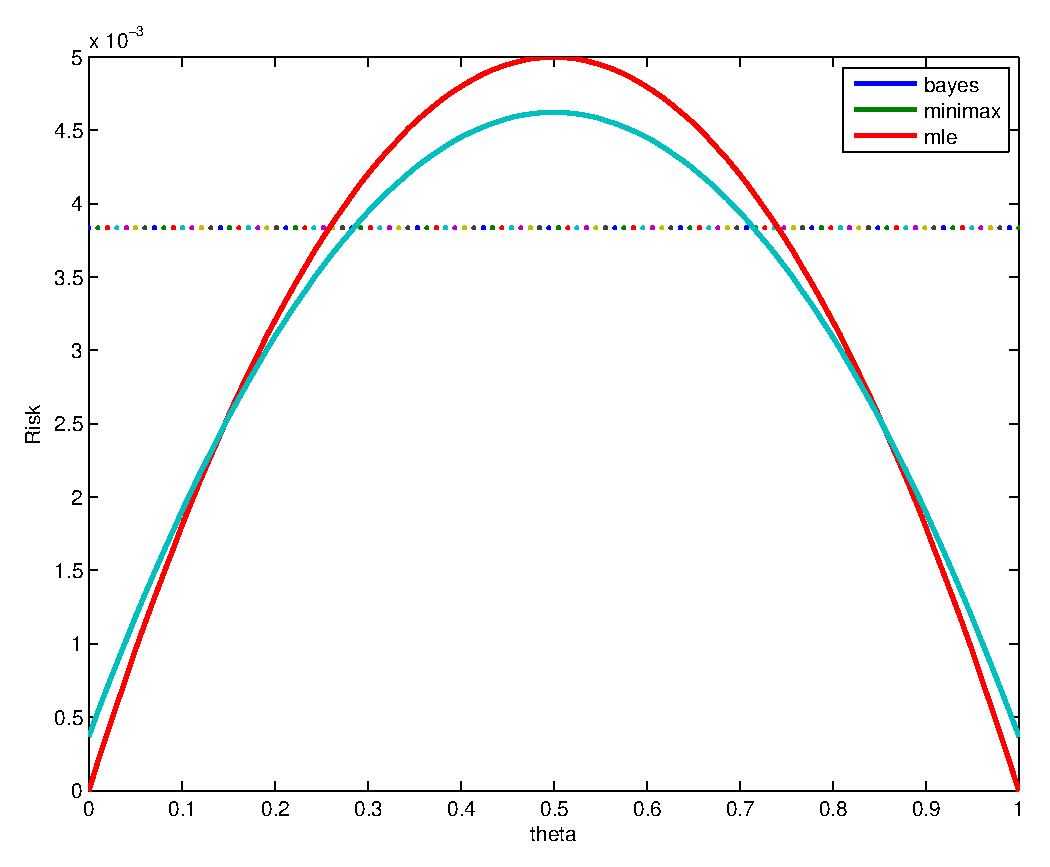
\includegraphics[width=3.5in]{2.eps}\\
\end{figure}
\end{itemize}
%%%%%%%%%%%%%%%%%%%%%%%%%%%%%%%%%%%%%%%%%%%%%%%%%%%%%%%%%%%%%%%%%%%%
% Reference
%%%%%%%%%%%%%%%%%%%%%%%%%%%%%%%%%%%%%%%%%%%%%%%%%%%%%%%%%%%%%%%%%%%%
%\begin{thebibliography}{1}

%\bibitem{BoydVandenberghe2004}
%S. Boyd and L. Vandenberghe, \emph{Convex Optimization}, Cambridge
%University Press, 2004.

%\end{thebibliography}
\end{document}
